\chapter{Di-$b$-jet Search: Outline and Event Selection}
\label{sec:evt}

In Chapter~\ref{sec:theo} it was shown that many Beyond Standard Model theories
predict new particles decaying to one or two $b$-quarks that could be produced by the LHC.
Chapters~\ref{sec:det},~\ref{sec:obj}~and~\ref{sec:trig}
described the detectors and reconstruction techniques used to observe such an event in the ATLAS detector.
Hence, I have now outlined the motivation and the tools required to perform
a search for resonances decaying to one or two $b$-jets,
an analysis that is called a di-$b$-jet search.

In Chapters~\ref{sec:evt},~\ref{sec:bkg}~and~\ref{sec:lim}
I will describe the di-$b$-jet search analysis using the ATLAS detector.
Each chapter will describe a separate part of the analysis,
the different parts are outlined Section~\ref{sec:evt-outline}.
The di-$b$-jet analysis is performed using three different data-sets,
the data-sets are described in Section~\ref{sec:evt-datasets}.

\section{Analysis Outline}
\label{sec:evt-outline}

The strategy used for the di-$b$-jet analysis
can be split up into broadly three parts.
A brief outline of the parts is given here,
and full detail can be fround in the relevant chapter.

\begin{itemize}[leftmargin=*]
\item\textbf{Di-$b$-jet Event Selection:} (\textit{Chapter~\ref{sec:evt}})\\
  The first step is to select events that are consistent with a resonance decaying to one or two $b$-quarks.
  Briefly, we will require two high-momentum jets and consider two $b$-tag categories;
  one where both jets have been $b$-tagged (2 $b$-tag) or where at least one jet has been $b$-tagged ($\geq$ 1 $b$-tag).
  The remainder of the chapter will focus on details of analysis selection;
  Section~\ref{sec:evt-datasets} will describe the data-sets used,
  Section~\ref{sec:evt-s+b} will describe the signal and backgrounds
  considered when defining the selections
  and Section~\ref{sec:evt-sel} will set out
  the details of the event selection used for each of the data-sets.
  \\
\item\textbf{Search Phase:} (\textit{Chapter~\ref{sec:bkg}})\\
  Once events have been selected the next part of the analysis aims to determine if there is
  is a new particle in the selected events; this step is known as the `search phase'.
  For this we will use the $m_{jj}$ spectrum, where $m_{jj}$ is the invariant mass of the two highest $p_T$ jets.
  A new particle will appear as a resonance (or `bump') on the smoothy falling
  $m_{jj}$ distibution from QCD multi-jet, as illustrated in Figure~\ref{fig:evt-dijet_schem}.
  A fit function is used to model the smoothly falling QCD background and a
  a model-independant search for for resonances is performed using the BumpHunter algorithm.
  Chapter~\ref{sec:bkg} contains a full description of the search phase strategy.
  %including tests of the fitting functions used and the results of the search phase in the data-sets considered.
  \\
  
  \begin{figure}[!hbt]
  \begin{center}
    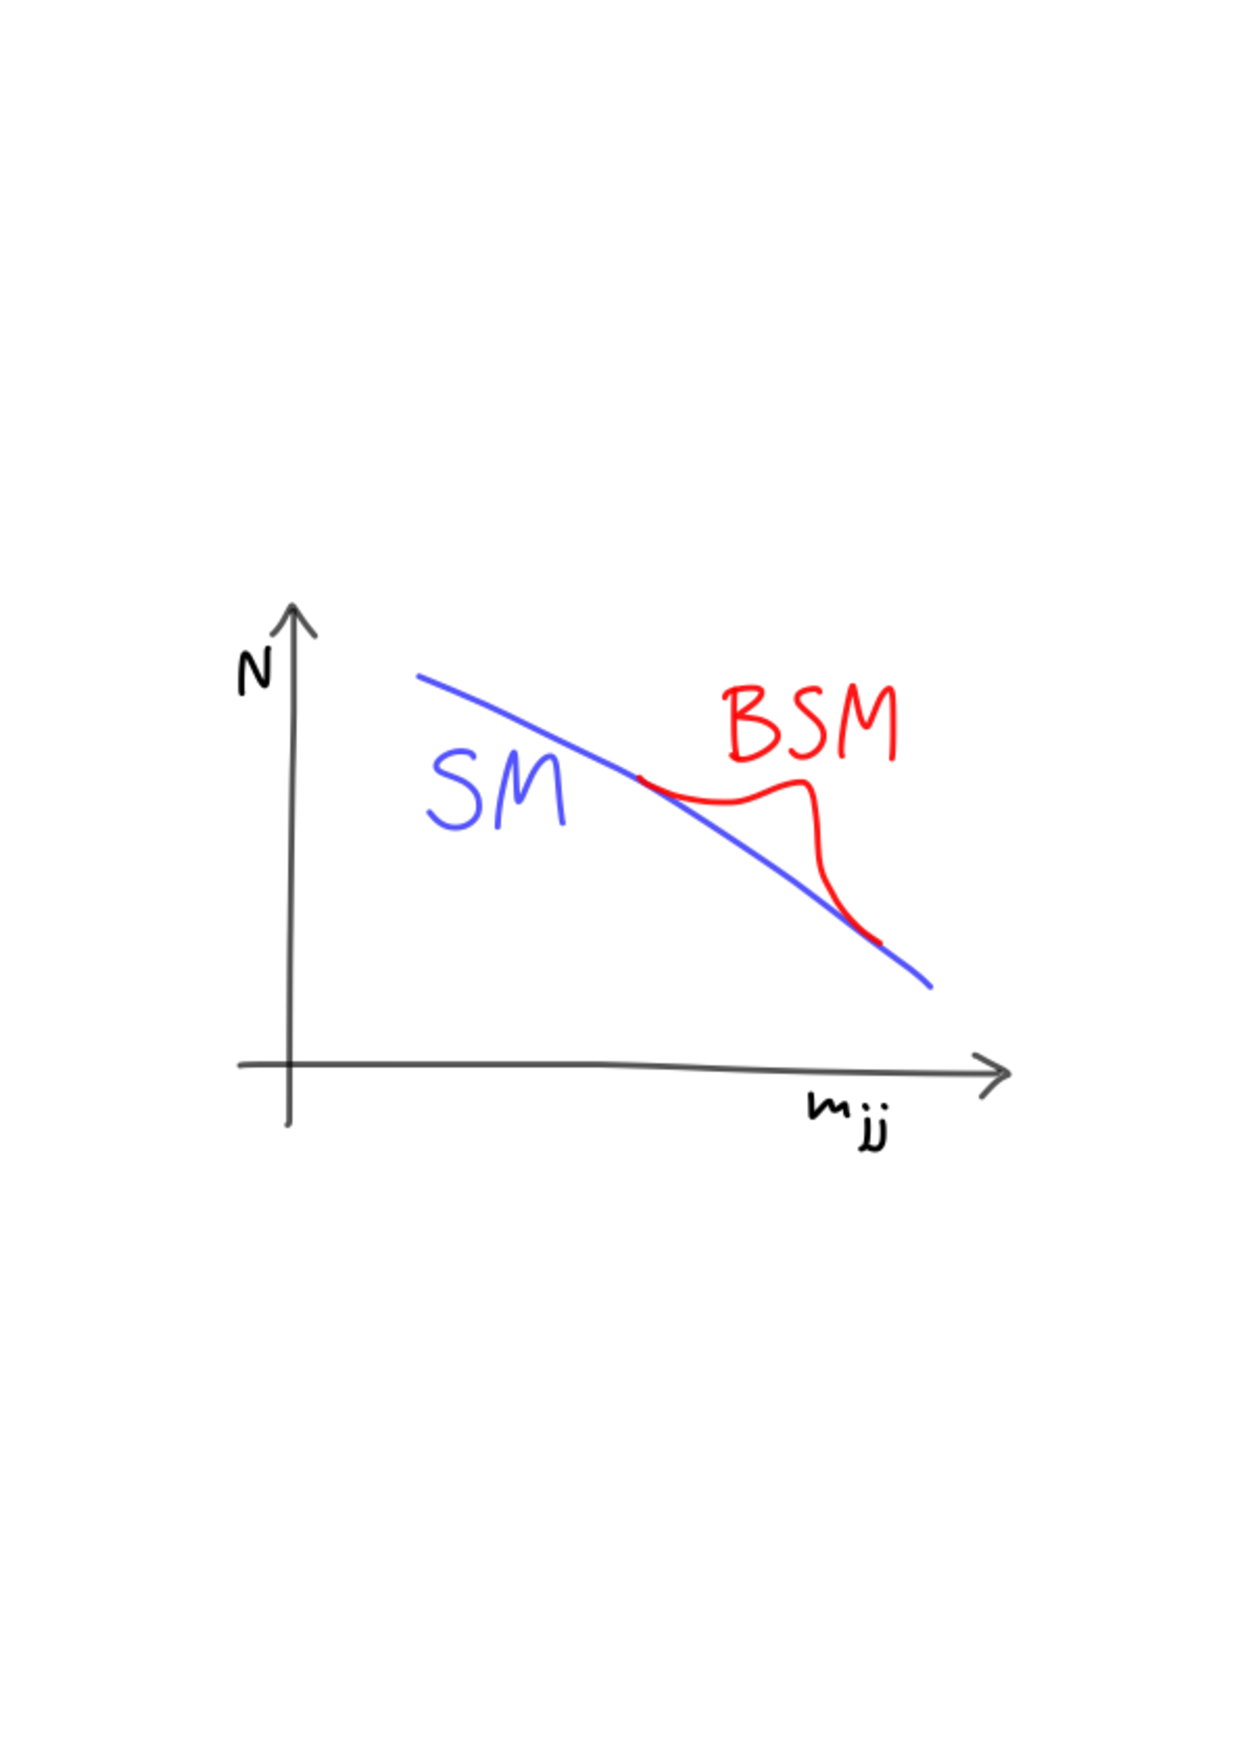
\includegraphics[width=0.5\linewidth, angle=0]{figs/Dibjet/Gen/dijet_schem.pdf}
  \end{center}
  \caption[A cartoon illustrating the use of dijet invariant mass ($m_{jj}$) distribution in the search phase of the di-$b$-jet analysis.
    Shown is the expected smoothly falling  distribution of multijet QCD (labelled as SM)
    and a resonance shape due to Beyond Standard Model particle (labelled as BSM)]
          {A cartoon illustrating the use of the dijet invariant mass ($m_{jj}$) distribution in the search phase of the di-$b$-jet analysis.
            Shown is the smoothly falling distribution from multijet QCD (SM)
            and a resonance shape caused by a Beyond Standard Model particle (BSM)~\textit{Reference Lene}.}
          \label{fig:evt-dijet_schem}
  \end{figure}
 
\item\textbf{Limit Setting:} (\textit{Chapter~\ref{sec:lim}})\\
  If, in the search phase stage of the analysis, no significant evidence of signal is
  found then it is desirible to quantify what cross-sections can be excluded as a result.
  95\% confidence lower mass limits are set on the two benchmark signals considered.
  The limit-setting methodology, description of systematics considered
  and final limit results in the data sets considered is contained in Chapter~\ref{sec:lim}.

\end{itemize}

\section{List of Datasets Used}
\label{sec:evt-datasets}

The di-$b$-jet analysis is performed in several iterations
as data is being collected, where each iteration uses a different data-set.
This is done for two reasons;
firstly it is important to know as soon as possible
if there is evidence of a new resonance as
this would affect our strategy moving forward and that of other analyses at ATLAS.
Secondly, this allows us to incrimentally
expand, adapt and improve this strategy in each iteration of the analysis.

In this thesis three different data-sets are considered by the di-$b$-jet analysis.
The overall analysis strategy is the same for each data-set,
so the interations are described together.
However, there are some significant differences in the details;
as such the during the analysis description it will be clearly labelled
which data-set is being referred to.

The data-sets are listed below,
and the trigger and Good Run List (GRL) used in each data-set is described.
The GRL is applied to remove events of low data-quality,
which is typically because an element of the detector was not operating optimally.
For example, data-taking periods where the inner-most layer of the inner detector,
the IBL, was not operating are removed as
this data-taking period had a lower $b$-tagging performance.
All quoted luminosities are given after the GRL has been applied.

\noindent
The data-sets are:

\begin{itemize}[leftmargin=*]
\item\textbf{Summer16+15}: \\
  The \verb|Summer16+15| data-set contains 13 TeV $pp$ collision data collected
  between January 2015 to July 2016 which has an intergrated luminosity 13.3~\ifb.
  The trigger used in this data-set, known as \verb|HLT_j380|,
  requires a trigger-level jet with $p_T >$ 380 GeV
  \footnote{\label{foot1} Further details of single-jet triggers is in Section~\ref{sec:trig-jet}.}.
  The analysis on this data-set was made published as a conference note~\cite{dibjet-ichep_conf}. \\
  
\item\textbf{Full16+15\_HighMass}:\\
  The \verb|Ful16+15_HighMass| data-set contains 13 TeV $pp$ collision data collected
  between January 2015 to December 2016, which has an intergrated luminosity of 36.1~\ifb.
  The trigger used in this data-set, known as \verb|HLT_j380|,
  requires a trigger-level jet with $p_T >$ 380 GeV
  \footnote{Again, see  Section~\ref{sec:trig-jet} for details on single-jet triggers.}.
  The analysis on this data-set has yet to be published.\\
  
\item\textbf{Full16\_LowMass}: \\
  The \verb|Full16_LowMass| data-set contains 13 TeV $pp$ collision data collected
  between January 2016 to December 2016, which has an intergrated luminosity of 24.3~\ifb.
  The trigger used in this data-set is known is a double $b$-jet trigger 
  which requires two trigger-level jets with $p_T >$ 150 GeV and $p_T >$ 50 GeV
  where both jets have been $b$-tagged at the trigger level
  \footnote{Further details of $b$-jet triggers and this particular trigger used in this analysis is in Section~\ref{sec:trig-bjet}.}.
  The \verb|Full16_LowMass| uses a $b$-jet trigger as the lower $p_T$ thresholds allow
  the analysis to probe a lower range of $m_{jj}$.
  This analysis did not combine data from 2015 as this used a significatly different $b$-trigger configuration.
  the \verb|Full16_LowMass| uses a $b$-jet trigger aware GRL, which in addition to the normal GRL,
  removed periods of data where the $b$-jet trigger was performing in a sub-optimal way,
  the GRL is described in Section~\ref{sec:trig-grl}.
  As the trigger uses is a double $b$-jet trigger, only the 2 $b$-tag category is considered.
  The analysis on this data-set has yet to be published.

\end{itemize}

\section{Backgrounds and Signal}
\label{sec:evt-s+b}

In the di-$b$-jet analysis selection we consider two
benchmark signal models and one background which will be dominant.
The signal models and dominant background are
used to optomise event selection, so I will describe
the signal and backgrounds considered here.

\begin{itemize}[leftmargin=*]
\item\textbf{Background: QCD Di-jet}: \\
  Section~\ref{sec:theo-qcd} discussed the details of QCD dijet production.
  In particular in Section~\ref{sec:theo-qcd-dijet_features} we noted that the
  relative strength of the strong force compared to other forces
  of the Standard Model means that
  QCD di-jet production would dominate other backgrounds in a di-$b$-jet event selection.
  Hence, this will be considered as our only background.
  A description of how the QCD di-jet background is modelled in this analysis is described in Chapter~\ref{sec:bkg}.\\

\item\textbf{Signal: $Z'$ Boson}: \\
  The $Z'$ boson is an additional gauge boson that can decay to two $b$-quarks,
  the theoretical $Z'$ models considered are
  described in detail in Section~\ref{sec:theo-bsm_zprime}.
  The $Z'$ boson provides a benchmark model in the 2 $b$-tag category.
  %in the case that both jets have been $b$-tagged.

  In the \verb|Summer16+15| data-set analysis we consider two $Z'$ boson models.
  The first is the Sequential Standard Model (SSM) $Z'$ where couplings to fermions
  are the same as the Standard Model and a leptophobic $Z'$ which couples to quarks
  as the Standard Model $Z'$, but does not couple to leptons.
  Monte-Carlo simulation is used to produce $m_{jj}$ signal templates;
  this is done using \textsc{Pythia8} ~\cite{dibjet-pythia8} with the A14~\cite{dibjet-a14} tune and the NNPDF23LO PDF set~\cite{dibjet-nnpdf}.
  Only decays to $b\bar{b}$ are simulated;
  other decays of the  $Z'$  are ignored such that our
  results are easier to interpret for other signal models decaying to pairs of $b$-quarks.
  Simulated $Z'$ boson templates are produced at mass points of
  1250, 1500, 1750, 2000, 2500, 3000, 4000 and 5000 GeV.
  
  \textbf{LM Fix Full addition}
  In the \verb|Full16+15_HighMass| data-set...
  Similarly the same models are considered in the \verb|Full16+15_LowMass|... \\

\item\textbf{Signal: $b^*$ Quark}: \\
  The $b^*$ quark is the third generation excited quark which results from
  quark compositeness models.
  The dominant decay mode of the  $b^*$ quark is to $bg$.
  The model considered is
  described in detail in Section~\ref{sec:theo-bsm_bstar}.
  The $b^*$ quark provides a benchmark model in the $\geq$1~$b$-tag category.
  %case that at least one of the jets has been $b$-tagged.
    
  
  In the \verb|Summer16+15| and \verb|Full16+15_HighMass|
  data-sets the same $b^*$ model is considered.
  Monte-Carlo simulation is used to produce a $b^*$ $m_{jj}$ signal template;
  again \textsc{Pythia8}~\cite{dibjet-pythia8} with the A14~\cite{dibjet-a14} tune and the NNPDF23LO PDF set~\cite{dibjet-nnpdf} is used.
  Decays to $bg$, $b\gamma$, $bZ_0$ and $tW^{-}$ are simulated.
  In the \verb|Full16+15_LowMass| data-set
  only the 2 $b$-tag category is used
  and as such that the $b^*$ model is not considered,
  further details can be found in Section~\ref{sec:evt-sel-btag}.
  Simulated $b^*$ quark templates are produced at mass points of
  1250, 1500, 1750, 2000, 2500, 3000, 4000 and 5000 GeV.
\end{itemize}

\section{Event Selection}
\label{sec:evt-sel}

The overall aim when designing the di-$b$-jet analysis event selection
is two-fold.
Firstly, events are selected to
maximise sensitivity to signal;
which we approximate in terms of $S$/$\sqrt{B}$,
where $S$ is the number of benchmark signal events and $B$ is the number of background events.
Secondly, we need to maintain the smoothly falling nature of the background,
which is the basic assumption of the background estimation strategy
described in Chapter~\ref{sec:bkg}.

The di-$b$-jet event selection is split up into three sections each described separately.
Firstly we select the jets to be considered (Section~\ref{sec:evt-sel-jets}),
then we apply a set of event-level kinematic cuts using the selected jets (Section~\ref{sec:evt-sel-event})
and finally we apply $b$-tagging to the jets (Section~\ref{sec:evt-sel-btag}).
In section~\ref{sec:evt-sel-acc} the total signal acceptance of the
event selection is evaluated.

Table~\ref{tab:evt} summarises the event selection for each of the
data-sets considered, for details refer to the text below.

\subsection{Jet Selection}
\label{sec:evt-sel-jets}

Jets are reconstructed using the anti-$k_T$ algorithm with $R=0.4$
and calibrated using the EM+JES scheme;
a full description of this is found in Section~\ref{sec:obj-jets}.

At least two jets are required in an event.
The two highest $p_T$ jets, referred to as the leading and subleading jet,
are the jets used throughout this analysis.
To reduce the number of fake jets from sources such as calorimeter noise
both jets are required to pass \textit{loose} jet cleaning cuts
based on the properties and distributions of the energy deposits in the calorimeter associated to the jet;
details can be found in~\cite{evt-jet_cleaning}.

Cuts are applied to the leading and subleading jet-$p_T$ such that events are on the trigger plateau;
the region where all events passing the offline jet-$p_T$ selection
would also pass the online jet-$p_T$ requriements of the trigger
\footnote{Using the definition from Section~\ref{sec:trig-bjet_eff}. Online refers to reconstructed objects used in the trigger decision,
  whilst offline refers to algorithms run after events have passed the trigger at the data-processing level. }.

For the \verb|Summer16+15| data-set; it is required that the leading jet has $p_T >$ 440 GeV to be on the trigger plateau of \verb|HLT_j380|.
This cut is derived by comparing the leading jet-$p_T$ distibutions of jets that pass the trigger, \verb|HLT_j380|,
relative to a benchmark trigger with a lower jet-$p_T$ threshold, \verb|L1_J75|.
Figure~\ref{fig:evt-jet_pt} shows this comparison in one run of data where \verb|L1_J75| was un-prescaled
\footnote{Un-prescaled means that the trigger accepts every event passing the trigger criteria};
in the ratio plot it is shown that for leading jet-$p_T >$ 440 GeV events are on the trigger plateau.
The subleading jet is required to have jet-$p_T >$ 60 GeV,
to avoid contamination from pile-up jets.
Both jets  are required to have $|\eta| <$ 2.4
such that the jets lies within the volume of the ATLAS pixel detector,
which is essential for optimal $b$-tagging performance.

\begin{figure}[!ht]
  \begin{center}
    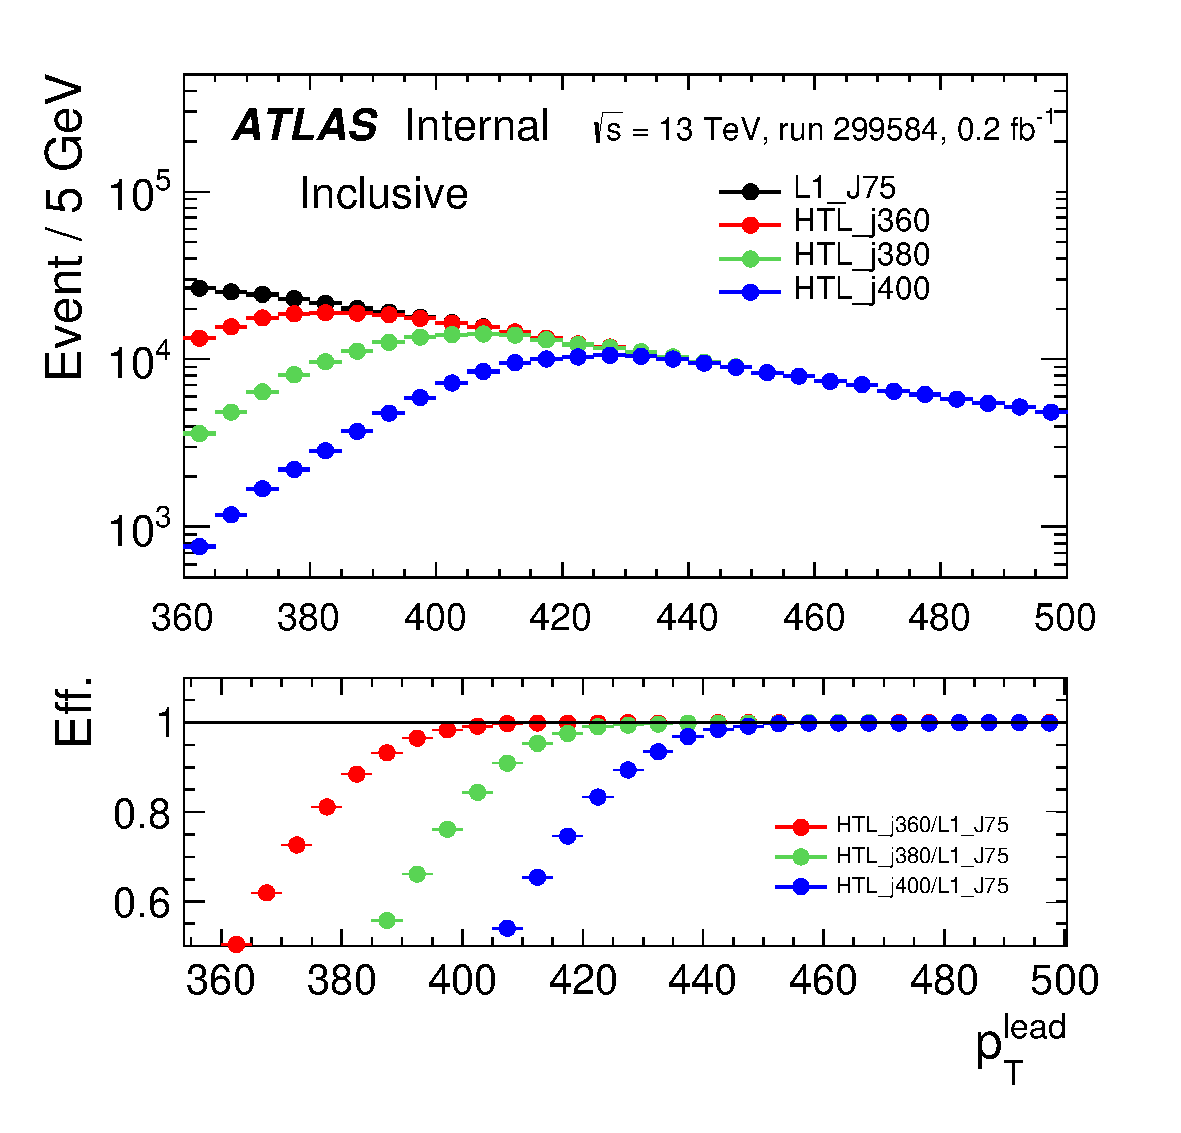
\includegraphics[width=0.8\linewidth, angle=0]{figs/Dibjet/ICHEP/evt-jet_pt.pdf}
  \end{center}
\caption[The comparisions of the leading jet-$p_T$ using unprescaled L1\_J75 trigger (black dots) to the HLT\_J360 trigger (red dots),
  HLT\_J380 trigger (green dots) and HLT\_J400 trigger (blue dots) in one run of 2016 data.
  The ratio with respect to L1\_J75 is shown in the lower panel.]
        {The comparisions of the leading jet-$p_T$ using an unprescaled L1\_J75 trigger (black dots) to the HLT\_J360 trigger (red dots),
          HLT\_J380 trigger (green dots) and HLT\_J400 trigger (blue dots) in one run of 2016 data.
          The ratio with respect to L1\_J75 is shown in the lower panel~\cite{dibjet-ichep_conf}.}
  \label{fig:evt-jet_pt}
\end{figure}

\subsection{Event Kinematics}
\label{sec:evt-sel-event}

\subsection{$b$-Tagging}
\label{sec:evt-sel-btag}

\subsection{Acceptance}
\label{sec:evt-sel-acc}

\begin{table}[!htb]
  \begin{tabular}{|c||c|c|c|}
    \hline
\thead{Cut}              &  \thead{Summer16+15} & \thead{Full16+15\_HighMass} & \thead{Full16+15\_LowMass} \\
\hline
%Trigger          & HLT\_380 & HLT\_380 & \makecell{ HLT\_j150\_bmv2c2060\_split\\\_j50\_bmv2c2060\_split} \\
Trigger          & Single-jet & Single-jet & \makecell{ Double $b$-jet} \\

\hline
Leading Jet-$p_T >$    &  440 GeV &  GeV &  GeV\\
Subleading Jet-$p_T >$ & 60 GeV & 60 GeV  &  GeV\\
Jet-$|\eta| <$   & 2.4 & 2.0 & 2.0 \\
\hline
$m_{jj} >$  & 1341 GeV & GeV & 500 GeV \\
$|y^*| <$ & 0.6 & 0.8 & 0.6  \\
\hline
$b$-Tagging OP & 85\% & 85\% & 70\%\\
$b$-Tag Categories & 2 and $\geq$1 & 2 and $\geq$1 & 2 \\
\hline
\end{tabular}
\centering
\caption{A summary of the key event selections applied in the di-$b$-jet analysis for each of the data-sets considered.}
\label{tab:evt}
\end{table}
